\chapter{Gate Array Reconfiguration}
\label{chap:Cap3}
\section{Full Reconfiguration}
La riprogrammabilità delle FPGA è la chiave per la loro adozione nei sistemi Cloud. In tal modo l'FPGA risulterà essere un sistema versatile, scalabile, efficiente ed ottimo per il cloud computing. Per la riprogrammazione delle FPGA SoC è possibile eseguire delle procedure automatiche, e non, per la riprogrammazione completa della Programmable Logic.

\subsection{FPGA Manager}
Esso bisogna che sia abilitato nella struttura del kernel, poichè è un insieme di API agnostiche che la loro chiamata ci permette di programmare, o riprogrammare, l'FPGA tramite un file binario.
\subsection{Creazione del file binario}
Per la creazione del file binario, si necessita un bitstream la quale generazione è discussa nell'appendice \ref{ExportVivado}.\\
Questa procedura necessita del tool bootgen, si rimanda a \ref{installazioneBoot} per l'installazione, il quale al fine di generare il file binario necessità uno file intermedio il Boot Image Format (BIF), questo file è cosi strutturato:
\begin{lstlisting}[language=sh, label=lst:C, caption={template file .bif}]
all:{./path/bitstream.bit}
\end{lstlisting}
Il file solitamente contiene tutte le fasi di boot ed eventuali partizioni dell'immagine.\\
Al termine di ciò sarà necessario caricare l'environment di lavoro di bootgen, semplicemente spostandosi nella cartella d'installazione ed eseguendo il seguente:
\begin{lstlisting}[language=sh, label=lst:C, caption={setup environment bootgen}]
source  settings64.sh
\end{lstlisting}
In questo modo tramite il comando 
\begin{lstlisting}[language=sh, label=lst:C, caption={setup environment bootgen}]
bootgen -image [/path/to/bifFile] -arch zynq -process_bitstream bin
\end{lstlisting}
All' appendice \ref{autoBOOT} è disponibile uno script in grado di automatizzare questo processo.
\section{Invocazione classe FPGA Manager}
Dopo la generazione del file binario, esso andrà copiato nella scheda SD in una qualsiasi partizione.\\
Al fine di abilitare la riprogrammazione completa della scheda sarà sfruttata la classe FPGA Manager, essa per l'abilitazione necessità alcuni comandi da eseguire all'interno della scheda\cite{PL}:
\begin{lstlisting}[language=sh, label=lst:C, caption={Abilitazione FPGA\_manager}]
echo 0 > /sys/class/fpga_manager/fpga0/flags
\end{lstlisting}
Questo comando imposta le Flags dell'fpga manager per accettare un nuovo bistream, quindi di fatto abilitando la riprogrammazione.\\
Di seguito bisognerà caricare il bitstream nella Programmable Logic
\begin{lstlisting}[language=sh, label=lst:C, caption={Caricamento bitstream nella Programmable Logic}]
mkdir -p /lib/firmware
cp [NomeBIN.bin] /lib/firmware/
\end{lstlisting}
Infine per effettuare la completa riprogrammazione è necessario puntare il nuovo file binario caricato nella PL, per far ciò è necessario comunicarlo al FPGA\_Manager
\begin{lstlisting}[language=sh, label=lst:C, caption={Comunicazione nuovo bitstream alla PL}]
echo [NomeBIN.bin] > /sys/class/fpga_manager/fpga0/firmware
\end{lstlisting}
La verifica dell'avvenuta riprogrammazione è visibile tramite un led on-board o tramite l'esecuzione di un sorgente che sfrutta il driver GPIO precedentemente discusso al capitolo \ref{comunicazioneCap}.\\
All'appendice \ref{Riprogrammazione} è possibile trovare uno script automatico per la riprogrammazione.
\section{Partial Reconfiguration}
\label{cap5}
Le FPGA, oltre la loro riprogrammazione, si rendono ancora più versatili tramite l'uso delle regioni. Quest'ultime rappresentano una parte di FPGA che può esser riprogrammata senza intaccare il resto della board, permettendo di avere molteplici acceleratori.\\
Le regioni definite nel seguente modo
\begin{figure}
    \centering
    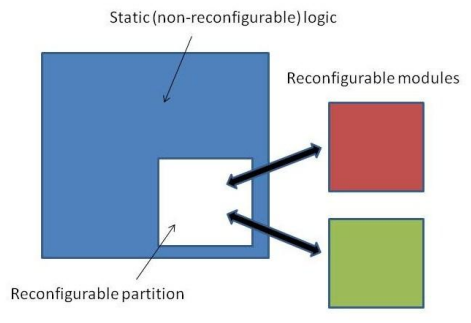
\includegraphics[width=0.4\textwidth]{images/PR1.png}
    \caption{Definizione regioni FPGA}
    \label{fig:my_label}
\end{figure}\\
Non tutte le regioni sono riprogrammabili, ma solo alcune. Queste vengono dette \textit{Partially Reconfigurable Region} (PRR). Questo modo di definire le FPGA rende ancora più conveniente la loro integrazione in un sistema IoT-Cloud.
\subsection{Place and Route per il Partial Bitstream}
La creazione di un Partial Bitstream, parte prima dalla progettazione dell'hardware, dove dovremmo descrivere, tramite Verilog o VHDL, un Intellectual Property(IP)\cite{PRRGIT}, un soft core che sia una blackbox, tramite essa sarà possibile effettuare il \textit{floorplanning}, esso è un tentativo di rappresentazione di come saranno piazzati i blocchi funzionali.
\begin{figure}
    \centering
    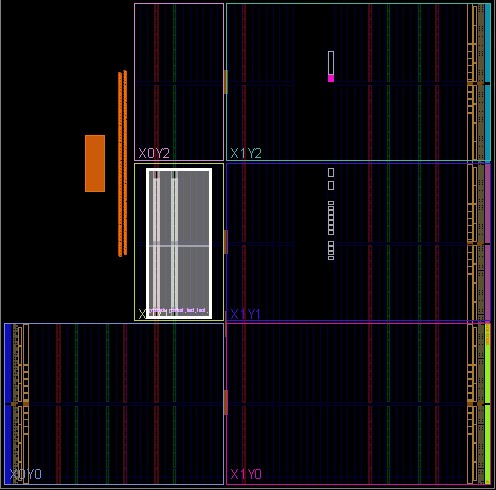
\includegraphics[width=0.4\textwidth]{images/Floor1.jpg}
    \caption{FloorPlanning in un FPGA Xilinx}
    \label{fig:my_label}
\end{figure}\\
Effettuato ciò potremmo effettuare il \textit{Place and Route}, generando cosi l'implementazione della scheda al fine di generare il \textit{Bitstream}\cite{PRR}. 
\subsection{Interfaccia per la riconfigurazione parziale}
Le FPGA SoC permettono la programmazione della Programmable Logic tramite il Processing System, esso si interfaccerà tramite l'interfaccia \textit{Device Configuration interface}(DevC), essa possiede un'interfaccia DMA che tramite il bus AXI trasferirà il partial bitstream ad una delle due \textit{Configuration Access Port}, rispettivamente \textit{Processor Configuration Access Port}(PCAP) e \textit{Internal Configuration Access Port} (ICAP).
\begin{figure}
    \centering
    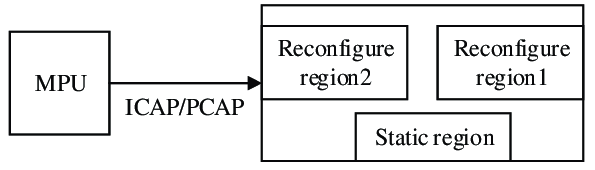
\includegraphics[width=0.4\textwidth]{images/PRR.png}
    \caption{Esempio di interfacciamento tra PS e PL per la riprogrammazione\cite{PRR2}}
    \label{fig:my_label}
\end{figure}\\
La loro coesistenza non è permessa dall'architettura, è possibile lo scambio tra le due interfacce anche runtime, tramite la modifica di un registro interno alla Processing System.\\
La \textit{Xilinx} garantisce un IP core \textit{AXI$\_$HWICAP}, che abilita la \textit{Partial Reconfiguration} tramite l'uso di \textit{ICAP}. Il processo di riprogrammazione parziale è stato svolto tramite l'uso di un controller chiamato \textit{ZyCap}\cite{PRR}
\begin{figure}
    \centering
    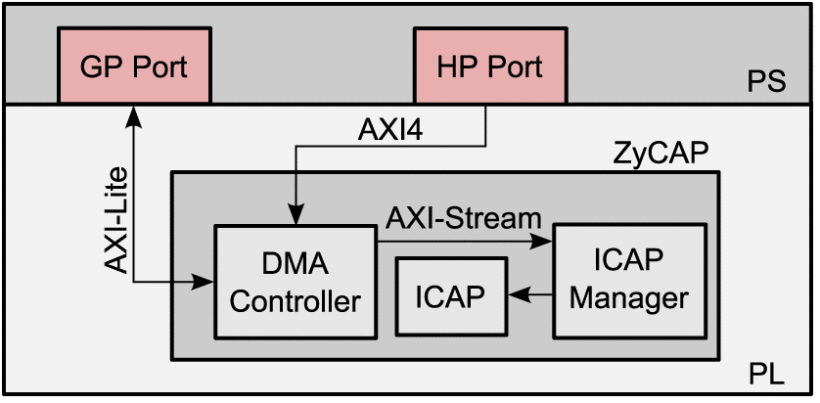
\includegraphics[width=0.4\textwidth]{images/ZyCap.png}
    \caption{Interfaccia tra PS e PL con il controller}
    \label{fig:my_label}
\end{figure}
\section{Problemi e possibili soluzioni}
Sfortunatamente l'architettura scelta al fine della realizzazione della tesi non supportava nativamente la \textit{Partial Reconfiguration}, rendendo impossibile la realizzazione di quest'ultima, anche causa un'obsoleta letteratura scientifica.\\
Il principale problema è dovuto dalla non completa integrazione di vivado con i meccanismi di sviluppo dei partial bitstream, poichè risulta impossibile esportare la definizione del hardware contenente tutte le informazioni inerenti al FPGA appena progettata, qualora si riuscisse ad esportare il file XSA sarà necessario creare il progetto su Vitis, ma le librerie usate in \cite{PRR} sono buona parte deprecate, rendendo inutile il processo di progettazione del codice per la riprogrammazione.\\
\subsection{Possibili soluzioni}
Alcuni possibili soluzioni potrebbero essere il cambio di architettura come ad esempio il passaggio a \textit{ZynqMP}, ma anche la creazione di un nuovo controller sulla base del \textit{Zycap}, quindi usando un \textit{AXI DMA} ed un controller per gli \textit{ICAP}. Ovviamente la creazione di un nuovo controller comporta la riscrittura del driver di riprogrammazione, che per alcuni tratti può esser basato su quello usato per il controllo del bus AXI, il driver dovrà necessariamente interfacciarsi con l'interfaccia \textit{DevC}, la quale però viene astratta tramite una libreria già fornita dalla \textit{Xilinx}.\\
Il metodo appena descritto può esser usato per effettuare una riprogrammazione \textit{BareMetal}, quindi senza la presenza di un sistema operativo lato PS, questo comporta l'introduzione di un elemento in più, assimilabile ad un Raspberry, che ospiterà l'agente \textit{Lightning-rod} per la connessione al Cloud.


